\begin{table*}[t]
\small
\singlespace
\centering
\caption{Resource Usage Results - where missing power results mean that the circuit could not be implemented on our power measurement platform (Xilinx ZC702)}
\label{tab:resources}
\tabcolsep=0.11cm
\begin{tabular}{@{}|l|l|l|l|l|l|l|l|l|l|l|l|l|@{}}
\toprule
                    & \multicolumn{4}{l|}{\textbf{Original}}                      & \multicolumn{4}{l|}{\textbf{StitchUp}}                      & \multicolumn{4}{l|}{\textbf{DMR}}                           \\ \midrule
\textbf{Bench}      & \textit{LUT} & \textit{REG} & \textit{DSP} &\textit{Pow mW} & \textit{LUT} & \textit{REG} & \textit{DSP} &\textit{Pow mW}& \textit{LUT} & \textit{REG} & \textit{DSP} & \textit{Pow mW}   \\ \midrule
\textit{aes}        & 47230        & 28152        & 0            & 299.346        & 47539        & 28800        & 0            & 316.186        & 90467        & 53944        & 0            & -              \\ \midrule
\textit{adpcm}      & 21050        & 16752        & 168          & 133.962        & 29599        & 29484        & 178          & 156.903        & 38664        & 31077        & 348          & -              \\ \midrule
\textit{blowfish}   & 97002        & 45320        & 0            & -              & 97440        & 46039        & 0            & -              & 194598       & 88268        & 0            & -              \\ \midrule
\textit{dfadd}      & 4639         & 4310         & 0            & 50.0916        & 5562         & 5095         & 0            & 54.224         & 6394         & 5754         & 0            & 58.114         \\ \midrule
\textit{dfdiv}      & 12144        & 13157        & 30           & 100.435        & 22254        & 23449        & 60           & 145.577        & 22811        & 23904        & 60           & 147.027        \\ \midrule
\textit{dfmul}      & 3348         & 3912         & 16           & 47.024         & 4553         & 4845         & 32           & 54.128         & 5105         & 5397         & 32           & 57.521         \\ \midrule
\textit{dfsin}      & 21343        & 20347        & 71           & 137.802        & 40928        & 38116        & 136          & 222.217        & 41136        & 38321        & 142          & -              \\ \midrule
\textit{gsm}        & 11953        & 9879         & 72           & 147.006        & 22049        & 17228        & 144          & 260.730        & 22399        & 17331        & 144          & 265.949        \\ \midrule
\textit{mips}       & 8278         & 6367         & 4            & 89.326         & 15639        & 10231        & 8            & 132.409        & 14304        & 10351        & 8            & 134.316        \\ \midrule
\textit{motion}     & 52665        & 26743        & 1            & -              & 104840       & 50719        & 1            & -              & 106986       & 51199        & 2            & -              \\ \midrule
\textit{sha}        & 9117         & 9287         & 3            & -              & 9491         & 10188        & 6            & -              & 16788        & 16189        & 6            & -               \\ \bottomrule
\end{tabular}
\end{table*}

To test the strengths and weaknesses of the StitchUp approach compared to DMR both techniques were evaluated on the CHStone benchmark suite.
In order to explore the effects of varying control-to-data ratio, we also evaluate the example code from 
Listing \ref{lst:DotProduct} while varying the degree of loop unrolling to increase data parallelism.
In all cases the resources in terms of LUTs, registers (REG), and DSPs were compared; and where the circuits could be implemented
on Zedboard/ZC702 devices, power results were obtained, and exhaustive error injection was performed.

\subsection{Unrolling Results}
\begin{figure}[t]
\centering
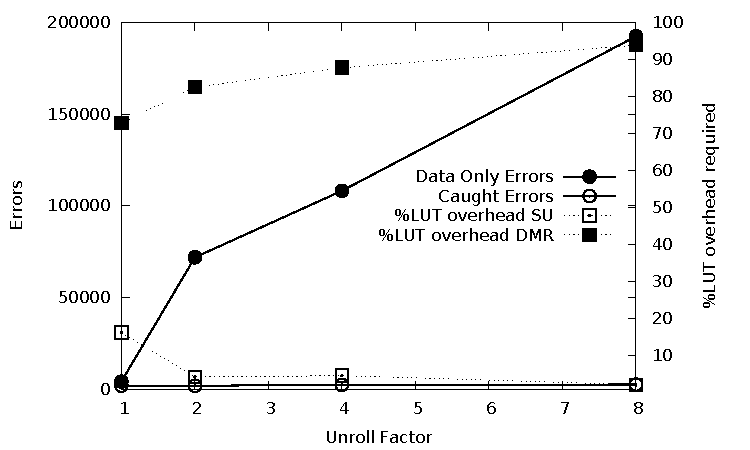
\includegraphics[width=3.25in]{./graphs/dp_unrolling_res.pdf}
\caption{Data Only Errors (DOEs) and Caught Errors (CEs) for a dot product with increasing loop unroll factors with StitchUp along with \%LUT overhead against DMR}
\label{fig:dp_unrolling_res}
\end{figure}

Figure \ref{fig:dp_unrolling_res} shows how the DOEs and CEs vary as the loop in Listing \ref{lst:DotProduct}
is unrolled.
Increasing the unroll factor reduces the control-to-data ratio since the number of basic blocks remains constant but the number of (data-flow)
only functional units instantiated in parallel increases.
This effect is observable in the results since the data only errors increase with the unroll factor but the number of caught errors
remains constant.
A similar trend can be observed for the percentage LUT overhead where the overhead for the DMR implementation
tends towards 100\% as the unroll factor increases, while the StitchUp overhead tends towards 0\%.
This tells us that as more non-control-structure instructions are executed in parallel, the overhead or
protection provided by the StitchUp replication is unaffected.

\subsection{Resource Overheads}
\renewcommand{\arraystretch}{0.8}

\begin{figure}[t]
\centering
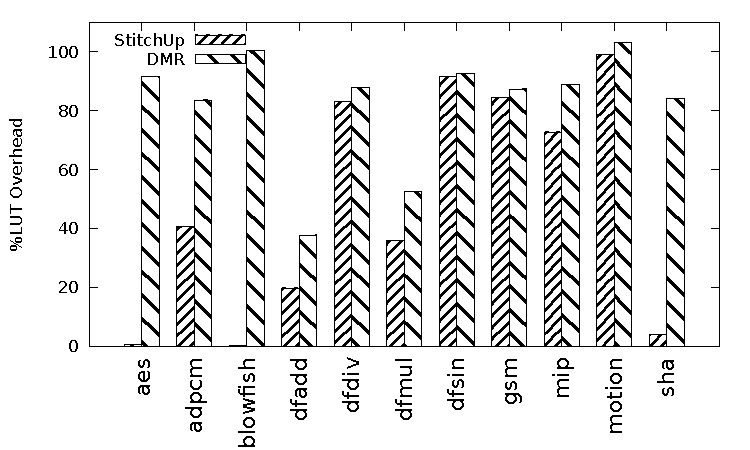
\includegraphics[width=3.25in]{./graphs/luts_res.pdf}
\caption{Comparison of \% LUT overheads required for both StitchUp and DMR}
\label{fig:lut_res}
\end{figure}

Table \ref{tab:resources} shows the required resources and power to implement
each of the CHStone benchmark circuits\footnote{with the exception of JPEG, which could not be routed onto our largest device}
with, no protection (original), StitchUp protection, and DMR protection.
Figure \ref{fig:lut_res} shows the relative percentage LUT overhead for the protection strategies on each circuit.
In cases where the control-flow and data-flow are decoupled, little replication is required - this effect can be seen in
the encryption benchmarks (aes, blowfish, sha) where replication can be as little as 1\% of the original circuit.
However there are other cases where protecting just the control flow structure results in essentially DMR, such as dfsin or dfdiv.
The amount of replication required by StitchUp is application dependant, however from these results we can see
that for a significant number of applications a low proportion of the original circuit needs to be replicated to
protect the control-flow structure.

%Power Results
\subsection{Power Results}
\begin{figure}[h]
\centering
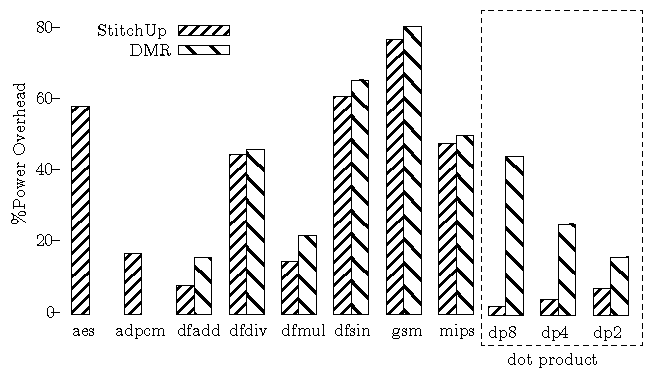
\includegraphics[width=3.5in]{./graphs/power_results.pdf}
\caption{Comparison of \% power overheads required for both StitchUp and DMR, where DMR power results for aes and adpcm could
not be obtained because they are too large to implement on our power measurement platform.}
\label{fig:power_res}
\end{figure}

Figure \ref{fig:power_res} shows the percentage power overheads for all circuits which can be implemented on the ZC702,
and when compared to the resource overhead results there is a close correlation between resources required and power consumed.
Along with some CHStone circuits the results for Listing \ref{lst:DotProduct} can be seen for an unroll factor 2 in dp2, unroll factor 4 in dp4,
and unroll factor 8 in dp8.
As the unroll factor increases and the ratio between control and data decreases the difference between the amount of power required by DMR and StitchUp also
increases, with StitchUp consuming less power as more work is performed in parallel.
This shows that not only does StitchUp have the potential to save area but that this also translates into a
saving in power.

\subsection{Fault Injection Results}

\begin{figure}[t]
\centering
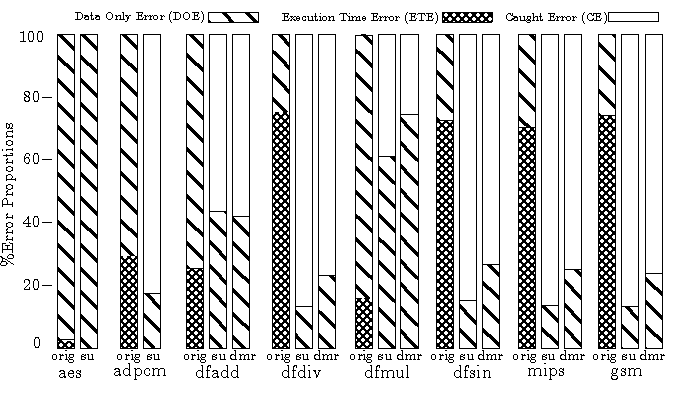
\includegraphics[width=3.5in]{./graphs/errors_res.pdf}
\caption{Error results for the CHStone benchmarks}
\label{fig:error_res}
\end{figure}

For every benchmarks possible to implement on the Zedboard device
exhaustive error injection was performed with each error categorised into either ETE, DOE, or CE.
Figure \ref{fig:error_res} shows the different proportions of these errors for each circuit, and in
all cases we can see that the ETE have been removed for both StitchUp and DMR.
Generally the proportion of the circuit that is replicated corresponds to the proportion of detected faults: for example aes
requires little replication but detects only ETEs; or dfsin, which requires a high proportion
of replication but also detects a high proportion of errors.
However there are some circuits between these extremes where the amount of replication returns a greater
proportion than expected of errors caught, such as adpcm where a 40\% replication results in 80\% of errors caught.
From these results not only can we see that StitchUp has the ability to remove all ETEs, but also
can catch a high proportion of errors relative to the amount of the original circuit that was replicated.
%\begin{table*}[t]
%\small
%\singlespace
%\centering
%\caption{Fault Injection Results}
%\label{tab:faults}
%\tabcolsep=0.11cm
%\begin{tabular}{|l|l|l|l|l|l|l|l|l|l|}
%\hline
%                    & \multicolumn{3}{l|}{\textbf{Original}} & \multicolumn{3}{l|}{\textbf{StitchUp}} & \multicolumn{3}{l|}{\textbf{DMR}} \\ \hline
%\textbf{Benchmarks} & \%ETE       & \%DOE       & \%CE       & \%ETE       & \%DOE       & \%CE       & \%ETE      & \%DOE     & \%CE     \\ \hline
%\textit{aes}        &             &             &            &             &             &            &            &           &          \\ \hline
%\textit{adpcm}      &             &             &            &             &             &            &            &           &          \\ \hline
%\textit{dfadd}      &             &             &            &             &             &            &            &           &          \\ \hline
%\textit{dfdiv}      &             &             &            &             &             &            &            &           &          \\ \hline
%\textit{dfmul}      &             &             &            &             &             &            &            &           &          \\ \hline
%\textit{dfsin}      &             &             &            &             &             &            &            &           &          \\ \hline
%\textit{gsm}        &             &             &            &             &             &            &            &           &          \\ \hline
%\textit{mips}       &             &             &            &             &             &            &            &           &          \\ \hline
%\textit{sha}        &             &             &            &             &             &            &            &           &          \\ \hline
%\end{tabular}
%\end{table*}

